\documentclass[twoside]{article}

\usepackage{lipsum}
\usepackage[sc]{mathpazo} 
\usepackage[T1]{fontenc} 
\linespread{1.05} 
\usepackage{microtype} % Slightly tweak font spacing for aesthetics
\usepackage{apacite}
\usepackage{graphicx}
\newenvironment{Figure}
  {\par\medskip\noindent\minipage{\linewidth}}
  {\endminipage\par\medskip}
  
\usepackage[hmarginratio=1:1,top=32mm,columnsep=20pt]{geometry} % Document margins
\usepackage{multicol} % Used for the two-column layout of the document
\usepackage[hang, small,labelfont=bf,up,textfont=it,up]{caption} % Custom captions under/above floats in tables or figures
\usepackage{booktabs} % Horizontal rules in tables
\usepackage{float} % Required for tables and figures in the multi-column environment - they need to be placed in specific locations with the [H] (e.g. \begin{table}[H])
\usepackage{hyperref} % For hyperlinks in the PDF

\usepackage{lettrine} % The lettrine is the first enlarged letter at the beginning of the text
\usepackage{paralist} % Used for the compactitem environment which makes bullet points with less space between them
\usepackage[authoryear,round,longnamesfirst]{natbib}

\usepackage{abstract} % Allows abstract customization
\renewcommand{\abstractnamefont}{\large\scshape\centering} % Set the "Abstract" text to bold
\renewcommand{\abstracttextfont}{\normalfont\itshape} % Set the abstract itself to small italic text
\renewcommand{\abstractname}{}    % clear the title
\renewcommand{\absnamepos}{empty}

\usepackage{titlesec} % Allows customization of titles
\renewcommand\thesection{\Roman{section}} % Roman numerals for the sections
\renewcommand\thesubsection{\Roman{subsection}} % Roman numerals for subsections
\titleformat{\section}[block]{\large\scshape\centering}{\thesection.}{1em}{} % Change the look of the section titles
\titleformat{\subsection}[block]{\large}{\thesubsection.}{1em}{} % Change the look of the section titles

\usepackage{fancyhdr} % Headers and footers
\pagestyle{fancy} % All pages have headers and footers
\fancyhead{} % Blank out the default header
\fancyfoot{} % Blank out the default footer
\fancyhead[C]{Emotional music computing $\bullet$ September 2015} % Custom header text
\fancyfoot[RO,LE]{\thepage} % Custom footer text


\title{\vspace{-15mm}\fontsize{24pt}{10pt}\selectfont\textbf{Emotional music computing}} % Article title
\author{
	\large
	\textsc{Karl-Arnold Bodarwé, Philipp Jean-Jacques, Jenny Noack}\\
	\normalsize University of Regensburg \\ % Your institution
	\vspace{-5mm}
}
\date{}

\hypersetup{
	pdfinfo={
		Author={Karl-Arnold Bodarwé, Philipp Jean-Jacques, Jenny Noack},
		Title={},
		Subject={...},
		Keywords={}
	}
}

\begin{document}
\maketitle
\thispagestyle{fancy}

\begin{abstract}
Music recommendation systems are well explored and commonly used but are normally based on
manually tagged parameters and simple similarity calculation. Our project proposes a recommendation system based on emotional computing, and automatic classification and feature extraction, which recommends music based on the emotion expressed by the song.\\
To achieve this goal a set of features is extracted from the song,\\ including the MFCC (mel-frequency cepstral coefficients) following the works of \citet{Mckinney2003} and a machine learning system is trained on a set of 500 Songs, which are categorized by emotion. The categorization of the song is performed manually by multiple persons to avoid error. The emotional categorization is performed using a modified version of the Tellegen-Watson-Clark emotion model \citep{Tellegen1999}, as proposed by \citet{Trohidis2011}. 
The System will be developed as desktop application. We hope to develop a system that can reliably determine similarities between the main emotion in multiple pieces of music, allowing the user to choose music by emotion.
\end{abstract}

\begin{multicols}{2} % Two-column layout throughout the main article text

\section{Introduction}
\lettrine[nindent=0em,lines=3]{I}n summer semester of 2015 we participated in a course on assistant systems at the University of Regensburg held by Professor Bernd Ludwig. During the semester our subject evolved into the project described below.\\
Musical Recommender systems are well known and widespread. Using methods such as tags or similar user behaviour, pieces of music can be recommended by a variety of features.\\
To try a new approach to this we decided to implement a recommendation system that classifies the main emotion of a certain piece of music by analyzing a set of features automatically extracted from the song. The extracted emotion is then used to recommend a song to the user, based on emotional similarity between songs or recommend the user a song by a certain emotion of choice.

\section{Related Work}
There have been various approaches on how to classify a piece of music by it’s emotion. There are different emotion models used as well as different feature extraction techniques.

\subsection{Emotion Models}
In multiple models emotion is mapped as a matrix where the axes relate to a certain emotional aspect and adjectives are placed in a circle inside the matrix to provide a guide. The number of axes varies from model to model and even in certain implementations of a model itself.\\
The Tellegen-Watson-Clark model, as used by Trohidis et al. has two axes labeled Positive Affect and Negative Affect which are used to show correlations between them and map emotions accordingly. Another dimension that can be derived from this model is the level of pleasantness of a certain emotion.\\

Other projects use the Valence Arousal model, a similar approach. The axes are labeled \textit{Valence} and \textit{Arousal}, with \textit{Valence} describing the happiness of the emotion and \textit{Arousal} describing the state of agitation entered by the emotion. The mapping of the adjectives to the matrix look similar to the Tellegen-Watson-Clark model, although the axes have different meanings.

\begin{Figure}
	\label{tellegen-nwatson-clark}
	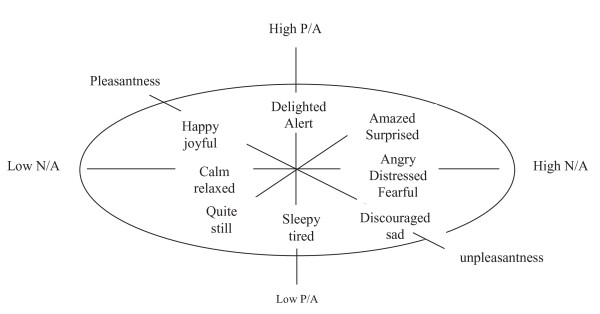
\includegraphics[width=\linewidth]{images/tellegen-watson-clark-model.jpg}
	\centering
	\textbf{The Tellegen-Watson-Clark model of mood} \citep{Tellegen1999}
\end{Figure}

\subsection{Feature Extraction and Classification}
Different researchers have tried different approaches to classification of music, not necessarily for classification of emotion. \citet{Mckinney2003} have proposed a method to automatically determine the genre of a certain piece of audio, including noise and speech. They tested different methods of classification against each other, resulting in good values for MFCC Analysis as well as Psychoacoustic features and a set of features called auditory filter temporal envelope, a set of bandpass filters which mimics the range of hearing of a human ear.\\

\citet{Li2003} give a comparison of classification techniques for automatic assignment of genres, including MFCC, FFT, Beat and Pitch, showing best results for FFT and MFCC, or a combination of these with other features. They make use of a Support Vector Machine for classifying, with good results.
\citet{Tzanetakis2001} also focus on the automatic classification of genres, focusing on the calculation of certain features such as STFT (short time fourier transform) and MFCC. The paper shows how to calculate the different features and explains the results. They find the best results when working with MFCC and STFT and identify genres that are harder to distinguish than others.

\section{Implementation}
\subsection{Assistence System}
\subsection{Emotion Model}
To be able to more easily distinguish between emotions, we decided to use a simplified version of the Tellegen-Watson-Clark model. We defined four emotional categories, marking the extreme ends of the graphs used in the model. The categories proposed in the Tellegen-Watson-Clark model have some adjectives that are very similar and difficult to distinguish especially when dealing with music as a carrier of emotion. Categories such as “calm-relaxing” and “quiet-still”, or “amazed-surprised” and “happy pleased” were combined into one category. The remaining categories are:

\begin{itemize}
	\item calm-relaxing
	\item happy-amazed
	\item angry-fearful
	\item sad-lonely
\end{itemize}

To create a set of training data to train a SVM on, we accumulated a collection of about 400 songs of various genre and artist, roughly sorted by their main emotion, by searching various online streaming and video platforms, such as Youtube and Spotify for playlists with tags fitting our emotional model.
The 400 songs were then classified by 3 independent raters into our four emotional categories. Afterwards Fleiss’ Kappa was calculated over the results. We decided to use only the songs classified with a Kappa value of 1. In total, 260 songs (61.32\%) were rated with a Kappa value of 1, 155 (36.56\%) had a value of 0.33 and 9 (2.12\%) were at Kappa value 0 with no consensus at all. Most of the disagreement (90 songs) were in categories “calm-relaxing” and “sad-lonely”, predicting difficulties in the differentiation of these categories.\\

To try to get an overview about useful features we processed a small sample of audio files with the jAudio feature extractor, extracting as many features as possible. We then used a two-step cluster analysis to analyze which features were actually useful and usable for our project. We found out that the MFCC, along with several low level parameters, was showing promising results and decided to use these parameters for classification.

\section{System}
The system was realized as a simple Audio Player, using ffmpeg for audio handling and javafx for the graphical user interface. The user interface provides a set of buttons associated with the emotions, which allow the user to filter the available songs through their emotion. A song is classified as soon as it is loaded into the player.

\begin{Figure}
	\label{screenshot}
	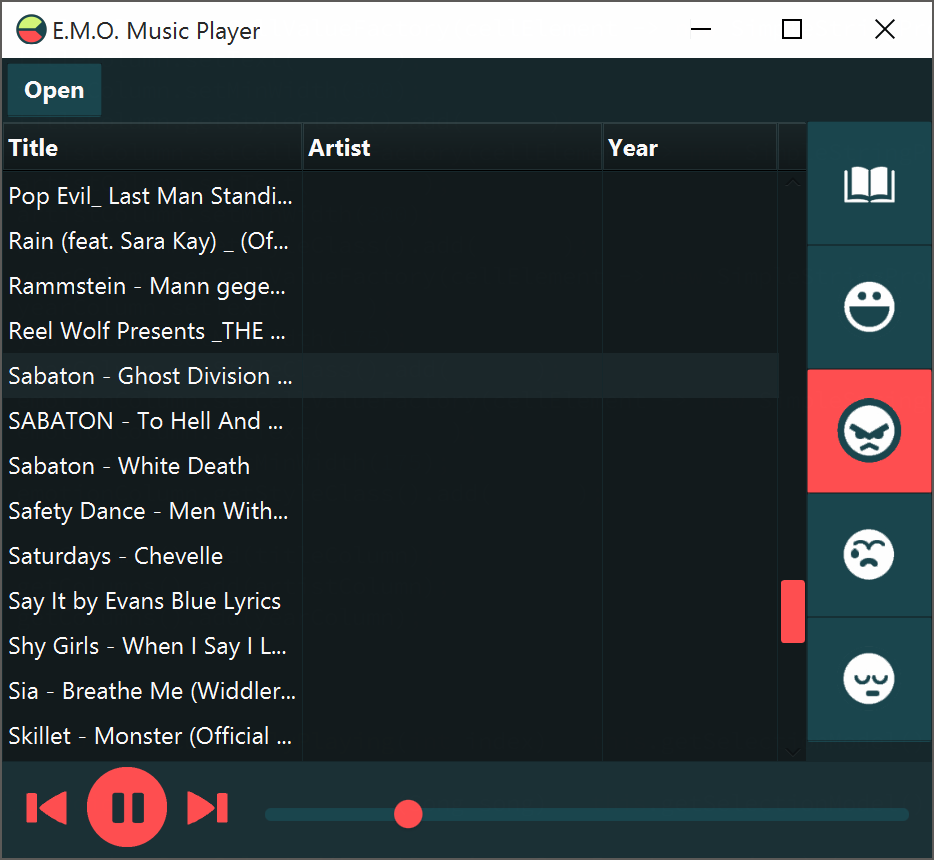
\includegraphics[width=\linewidth]{images/screenshot.png}
	\centering
	\textbf{User interface of the music player}
\end{Figure}
\vspace*{10pt}

During the development of the feature extraction process several approaches were tested for performance and format compatibility. Since the audio processing library \textit{MARSYAS} \citep{Tzanetakis1999} is written in C++ it was not considered for the player. \textit{TarsosDSP} \citep{Six2014} is another audio processing library with focus on real time audio processing. It is written in Java but does not support the mp3 format. The last library considered was \textit{jAudio} \citep{McEnnis2005}, a library specifically developed for feature extraction. This library is also written in Java and supports both wav and mp3 formats and was therefore chosen over the other two.\\

% Technische Beschreibung des Systems
% Welche Features wurden verwendet => MFCC(Mean, SD), RMS, Chroma
% Classifier: Naive Bayes => hat einfach besser funktioniert. SVM oder Regression/Cluster waren schlechter
% Beschreibung des Players

\section{Results}
To test and rate the quality of our classification model, it was tested using the cross validation method on the training data using ten folds. Our findings are as follows:...

% hier statistiken

In the process of the project, we have come to a few conclusions regarding methods and tools. We at first used the jAudio library to get an overview of available features, but struggled with the documentation of the code. While jAudio has an easy to use stand-alone feature extractor, which can create great amounts of usable data in little time, the possibility to embed the library into a system is lacking.
\\
\section{Conclusion}

% je nachedm was das ergebnis ist

\bibliographystyle{apacite}
\bibliography{literature}

\end{multicols}
\end{document}
